%% Optics Express manuscript -- Optica Publishing Group universal template (optica-article.cls)
%% Compile with pdfLaTeX + BibTeX.  Files needed alongside this one: optica-article.cls, styles/opticajournal.sty,
%% opticajnl.bst, jabbrv.sty, jabbrv-ltwa-all.ldf, jabbrv-ltwa-en.ldf (all shipped with the Overleaf template), refs.bib, figs/.
%% v3 (8-page revision, writer loop 2). Figures fig1_five_layer ... fig7_qas_nk are regenerated by notebooks/nb1..nb6;
%% every number is taken from results/nb*.json (including the loop1_checks keys; PI/Si = nb2 loop1_checks/fig2b_variant).
%% fig1_five_layer is not included (R4/R14: dropped for the 8-page budget; one sentence in Sec. 4).
\documentclass{optica-article}
\journal{opticajournal}          % use \journal{oe} if your template version ships an Optics Express style file
\articletype{Research Article}
\setcopyright{Optica Publishing Group under the terms of the Optica Open Access Publishing Agreement}

\usepackage{amsmath,bm}
\usepackage{booktabs,multirow}
\usepackage{siunitx}\sisetup{detect-all,range-phrase=--,range-units=single}
\usepackage{xcolor}\newcommand{\todo}[1]{\textcolor{red}{#1}}
\newcommand{\nb}[1]{\todo{\textsuperscript{[nb#1]}}}   % number awaiting results/nb#1*.json (unused)
\newcommand{\XX}{\todo{XX}}                               % placeholder for a number not yet available (unused)
\graphicspath{{figs/}}
% float placement: allow pages that are mostly floats
\renewcommand{\topfraction}{0.95}\renewcommand{\bottomfraction}{0.9}\renewcommand{\textfraction}{0.03}
\renewcommand{\floatpagefraction}{0.95}\setcounter{topnumber}{3}\setcounter{bottomnumber}{3}\setcounter{totalnumber}{5}
\setlength{\textfloatsep}{6pt plus 2pt minus 2pt}\setlength{\intextsep}{6pt plus 2pt minus 2pt}\setlength{\floatsep}{6pt plus 2pt minus 2pt}\setlength{\abovecaptionskip}{3pt}\setlength{\belowcaptionskip}{0pt}
\widowpenalty=150\clubpenalty=150\raggedbottom\allowdisplaybreaks
\captionsetup{width=\linewidth}  % captions at full text width (class default 4.25in) to meet the 8-page budget
\newcommand{\kap}{\kappa}
\newcommand{\Lt}{\mathcal{L}}
% layer subscripts: q = quartz, Si = silicon, PI = polyimide (figure axis labels of Figs. 4, 5 use 1 = quartz, 2 = Si)
\newcommand{\nq}{n_{\mathrm q}}\newcommand{\kq}{\kap_{\mathrm q}}\newcommand{\dq}{d_{\mathrm q}}
\newcommand{\nS}{n_{\mathrm{Si}}}\newcommand{\kS}{\kap_{\mathrm{Si}}}\newcommand{\dS}{d_{\mathrm{Si}}}

\begin{document}

\title{Terahertz multilayer material parameter extraction with a differentiable transfer-matrix model: what the loss landscape says about what can be measured}

\author{Theo Smith,\authormark{1} Arta Latifi,\authormark{2} Nicholas T. Klokkou,\authormark{1} Ben Beddoes,\authormark{1} Jon Gorecki,\authormark{2} Georgios D. Barmparis,\authormark{3} and Vasilis Apostolopoulos\authormark{*,3,1}}

\address{\authormark{1}School of Physics and Astronomy, University of Southampton, Southampton SO17 1BJ, United Kingdom\\
\authormark{2}Royal School of Mines, Imperial College London, London SW7 2AZ, United Kingdom\\
\authormark{3}Laser and THz Laboratory, Department of Physics, University of Crete, Heraklion 70013, Greece\\
\authormark{4}Twenty-One Semiconductors GmbH, Neckartenzlingen, Germany\\
\authormark{5}Optoelectronics Research Centre, University of Southampton, Southampton SO17 1BJ, United Kingdom\\
\todo{[authors, affiliations (4, 5 unassigned) and order to be confirmed]}}

\email{\authormark{*}v.apostolopoulos@physics.uoc.gr}

\begin{abstract}
Terahertz time-domain spectroscopy can return the thickness and complex refractive index of each layer of a stratified sample from one transmitted pulse, but the inverse problem is unstable for thin or multiple layers. We fit a differentiable transfer-matrix model to the measured pulse with Adam and L-BFGS and ask what the data determine. Simulations with a measured reference pulse show noise-limited recovery of a thin film down to a round trip comparable with the pulse duration. For a polyimide film on silicon a time offset between reference and sample must be fitted, so absolute thicknesses rest on time zero. On a quartz/silicon bilayer the pulse timings fix each layer's optical thickness reproducibly to \SI{0.1}{\percent} within one interface model; an interface gap shifts it by \SI{1}{\percent}. Two soft directions remain, a transfer of thickness and a split of the attenuation between the layers. Adam drifts along the latter for most of its budget, and the sign of the silicon extinction coefficient depends on the estimator; a softplus constraint imposes the physical sign, $\kap\ge0$. L-BFGS needs no step-size tuning but stalls at a kink of the mean-absolute loss. A six-knot dispersive model determines an air gap eight times better than either plate.
\end{abstract}

% =====================================================================================
\section{Introduction}
Terahertz time-domain spectroscopy records a picosecond pulse as a time-resolved field through air (the reference) and through the sample; for a thick slab the complex index follows stably, frequency by frequency \cite{Grischkowsky1990,Duvillaret1996,Naftaly2007,Withayachumnankul2008}. For thin or multiple layers the delayed replicas of the pulse from internal reflections (Fabry--P\'erot echoes) overlap and the problem becomes non-convex \cite{Scheller2009}, precisely where thickness gauging is in demand \cite{Yasui2005}; fitting the whole time trace \cite{Peretti2019} avoids phase unwrapping but not the non-convexity.

We treat the extraction as an inverse problem \cite{Aster2018}, fitting a differentiable transfer-matrix method (TMM) \cite{BornWolf1999,Paszke2019} for thickness $d$, index $n$ and extinction coefficient $\kap$ of every layer with Adam \cite{Kingma2017} or limited-memory BFGS (L-BFGS) \cite{Nocedal2006}. We show (i) how thin a film can be extracted at the noise limit (Section~\ref{sec:sim}), (ii) what a bilayer fit's loss landscape determines (Section~\ref{sec:landscape}), (iii) how Adam and L-BFGS cross it (Section~\ref{sec:lbfgs}), and (iv) what a dispersive model adds (Section~\ref{sec:disp}).

\begin{figure}[b]\centering
  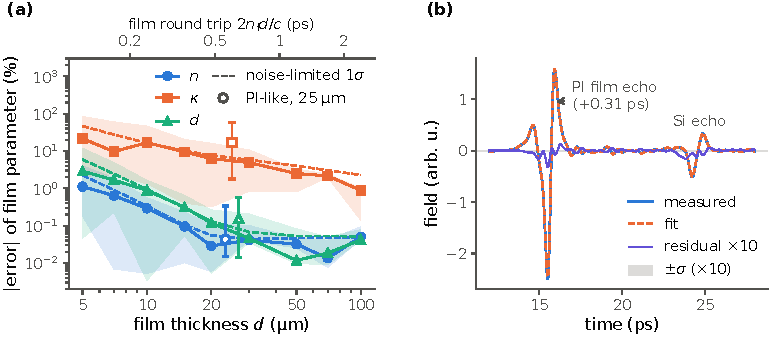
\includegraphics[width=\linewidth]{fig2_thin_film}
  \caption{Thin film on a substrate. (a) Simulated thickness sweep (film $n_{\mathrm f}=3.6$, $\kap=0.0203$; substrate $n=2.213$, $\kap=0.0125$, $d=\SI{496}{\micro\metre}$; $\sigma=\num{1.58e-3}$, peak/$\sigma=2.1\times10^3$). Symbols: median error; bands: range; 13 noise draws (5--\SI{20}{\micro\metre}), 3 above; dashed: noise-limited (Cram\'er--Rao, CR) $1\sigma$. Top axis: simulated film only. Hollow symbols (offset for clarity): PI-like film ($n=1.72$, $\kap=0.01$ on Si, five draws) at \SI{25}{\micro\metre} (round trip \SI{0.29}{\pico\second}). (b) Polyimide on Si fitted with a free time offset $\tau$ ($\sigma=\num{1.35e-3}$); residual and $\pm\sigma$ band $\times10$.}
  \label{fig:limits}
\end{figure}

% =====================================================================================
\section{Forward model: transfer-matrix method}\label{sec:tmm}
For a pulse entering layer $j$ of complex index $\tilde n_j = n_j - i\kap_j$ and thickness $d_j$ from a medium of index $n_{\mathrm a}$, with $D_j=\omega d_j/c$ and $g_j^{\pm}=\tfrac12\left(n_{\mathrm a}/\tilde n_j\pm\tilde n_j/n_{\mathrm a}\right)$, field continuity gives \cite{BornWolf1999}
\begin{equation}
  r_j = \frac{ig_j^{-}\sin(\tilde n_j D_j)}{\cos(\tilde n_j D_j)+ig_j^{+}\sin(\tilde n_j D_j)}, \label{eq:r}\qquad
  t_j = \frac{e^{in_{\mathrm a}D_j}}{\cos(\tilde n_j D_j)+ig_j^{+}\sin(\tilde n_j D_j)},
\end{equation}
where the factor $e^{in_{\mathrm a}D_j}$ references $t_j$ to the same thickness of ambient. The slabs are combined recursively into the stack transmission $T(\omega)$, since zero-thickness ambient layers between slabs leave the characteristic matrix unchanged; the sample pulse is the reference $x(t)$ filtered by $T$,
\begin{equation}
  y(t)=\mathcal{F}^{-1}\!\left[T(\omega)\,\mathcal{F}[x(t)]\right],
  \label{eq:forward}
\end{equation}
on a zero-padded grid ($4L$ points for $L$ samples); every operation is differentiable.

% =====================================================================================
\section{Inverse problem: parameters, loss, noise and optimisers}\label{sec:inverse}
Until Section~\ref{sec:disp} the indices are frequency-independent; the echo timing of a layer measures its optical thickness $n_jd_j$. We use a robust pipeline for the simulations and the polyimide film, and a plain one for quartz/Si, whose slow phase we want to see. In the robust one the optimiser variables $u$ enter as $n=n_{\mathrm{st}}+0.1u$, $\kap=\kap_{\mathrm{st}}+0.005u$, $d=d_{\mathrm{st}}e^{0.1u}$ about the start values. L-BFGS runs coarse to fine, on traces low-pass filtered at \SIlist{0.25;0.5;1}{THz} and then on the full band; the loss is the root-mean-square error (rMSE) plus a hinge penalty $\sum_j\max(0,-\kap_j)$ (weight 1) against gain. The sweep uses five starts in a box centred on the truth ($n\pm0.5$, $\kap\pm0.01$, $d\times[0.5,1.5]$), the PI fit the nominal guess and seven random starts. For quartz/Si the optimiser variables are the ratios $\theta_i=p_i/p_i^{(0)}$ of each parameter to its start value (Table~\ref{tab:exp}), and the loss is
\begin{equation}
  \Lt_{\mathrm{exp}}(\theta)=\frac{1}{L}\sum_k\left|\hat y_k-y_k\right| + \frac{1}{L}\sum_k \ln\cosh\!\left(\hat y_k-y_k\right).
  \label{eq:lossexp}
\end{equation}
Its first term is the mean absolute error (MAE); the log-cosh term, half the mean square for residuals $\ll1$, adds \SI{1.6}{\percent} to the loss at the Adam end point.

The noise floor $\sigma$ is the standard deviation of the first \SI{10}{\pico\second} of the sample trace (reference trace for the sweep, which has none). This noise is bursty, its white part 6 to 72 times smaller: $\sigma$ is a bookkeeping scale, not a white-noise level.

Adam keeps moving averages $\hat m_t$, $\hat v_t$ of the gradient and its square, updating $\theta_{t+1}=\theta_t-\eta\,\hat m_t/(\sqrt{\hat v_t}+\epsilon)$, so every parameter moves at about the rate $\eta$ however weakly the loss depends on it. L-BFGS builds a curvature estimate from the gradient history (strong-Wolfe line search). The lowest-loss start is kept; Bayesian optimisation of the start, used earlier, was abandoned as for five-layer stacks it led to wrong echo assignments at higher cost.

% =====================================================================================
\section{Simulated extractions and a thin film}\label{sec:sim}
For a thin film on a thick substrate we sweep the film thickness with the reference of Section~\ref{sec:exp}, adding white noise to the sample (Fig.~\ref{fig:limits}(a)). The scatter equals the CR bound (Section~\ref{sec:cr}) within \SI{26}{\percent} in $n$, $d$, without bias: the sweep is noise-limited. For this film the median error in $d$ exceeds \SI{1}{\percent} between 7 and \SI{10}{\micro\metre}, where the round trip falls below two thirds of the reference full width at half maximum (FWHM, \SI{0.36}{\pico\second}) and the film echo merges with the main pulse.

The experimental counterpart is a spin-coated polyimide (PI) film (HD Microsystems PI-2525) on silicon \todo{[sample details; float-zone Si?; profilometer uncertainty and stylus-to-THz-spot offset]} (Table~\ref{tab:pi}). On a common time axis the fit returns an impossible $\nS=3.26$ \cite{Dai2004}, which absorbs a timing error: every start conserves the pulse delay and the Si echo spacing. We therefore shift and scale the reference by $\tau$ and $a$, for drifts of the delay-stage zero and source power between scans \SI{23}{\minute} apart: $y=a\,\mathcal F^{-1}[T\,\mathcal F[x]\,e^{-i\omega\tau}]$ ($\tau<0$: early sample). As the timings fix every $n_jd_j$ (Section~\ref{sec:sens}), \SI{10}{\femto\second} of $\tau$ moves $d_{\mathrm{PI}}+\dS$ by \SI{3}{\micro\metre}. The misfit falls by over a third, $\nS$ comes within \SI{0.4}{\percent} of the literature value and $d_{\mathrm{PI}}$ lies \SI{2}{\percent} above the profilometer value, with $\nS$ free or fixed; the two best starts agree on $n_{\mathrm{PI}}d_{\mathrm{PI}}$ to \SI{0.2}{\percent}. The fits with and without $\tau$ put the attenuation in different layers, so its split is not determined. A PI-like simulation recovers a \SI{25}{\micro\metre} film to \SI{0.16}{\percent} in $d$ (its \SI{1}{\percent} limit is at 10--\SI{15}{\micro\metre}), so the \SI{2}{\percent} found here is systematic.
% AUTHOR NOTE (not for print): the PI sample will be re-measured (reference and sample scans close in time, purged);
% Fig. 1(b) and Table 1 will then be updated from the new data (R27).

\begin{table}[!htb]\centering\scriptsize\setlength{\tabcolsep}{3.2pt}
  \caption{Polyimide on silicon ($d$ in \si{\micro\metre}, $\tau$ in \si{\femto\second}): best of eight starts with free $\tau$, $a$; CR bound (none for $\kS$, at $\kap\ge0$); fit without $\tau$, $a$; independent values ($^a$white light, \SI{633}{\nano\metre}; $^b$profilometer; $^c$Ref.~\cite{Dai2004}; $^d$product of the values marked $^a$ and $^b$, a guide only). With $\nS=3.4175$ fixed: $d_{\mathrm{PI}}=25.25$, $\tau=-65.4$, rMSE $1.70\sigma$. The 2 of 8 starts within \SI{0.5}{\percent} of the best rMSE agree on $n_{\mathrm{PI}}d_{\mathrm{PI}}$ to \SI{0.22}{\percent}.}
  \label{tab:pi}
  \begin{tabular}{l cccccc c cc c}\toprule
    & $n_{\mathrm{PI}}$ & $\kap_{\mathrm{PI}}$ & $d_{\mathrm{PI}}$ & $\nS$ & $\kS$ & $\dS$ & $n_{\mathrm{PI}}d_{\mathrm{PI}}$ & $\tau$ & $a$ & rMSE$/\sigma$\\\midrule
    $\tau$, $a$ free & 1.784 & 0.029 & 25.24 & 3.430 & at bound & 380.2 & 45.01 & $-70.1$ & 1.024 & 1.70\\
    CR bound & 0.0019 & 0.0007 & 0.038 & 0.0022 & -- & 0.24 & 0.037 & 0.83 & 0.0005 & \\
    no $\tau$, $a$ & 1.712 & at bound & 25.84 & 3.259 & 0.0006 & 400.2 & 44.26 & -- & -- & 2.69\\\midrule
    independent & $1.726^a$ & & $24.7^b$ & $3.4175^c$ & & & $42.63^d$ & & & \\
    \bottomrule
  \end{tabular}
\end{table}

% =====================================================================================
\section{Experimental extraction: quartz on silicon}\label{sec:exp}
A quartz plate (q) and a silicon wafer (Si), clamped in contact without adhesive \todo{[nominal and mechanical thicknesses, supplier]}, were measured under nitrogen (Fig.~\ref{fig:expfit}) and fitted with Adam ($\eta=10^{-4}$) from three starts for $2\times10^4$ iterations. The end points spread by $2.3\times10^{-4}$ in $\nq$ and \SI{0.16}{\micro\metre} in $\dq$ and $\dS$, along a soft direction (Section~\ref{sec:sens}); three times as many iterations change the loss by $<\SI{0.02}{\percent}$: an Adam end point, not an optimum. The quartz index is that of fused silica \cite{Grischkowsky1990,Naftaly2007} \todo{[confirm sample material]}. $\nS$ is \SI{0.9}{\percent} above the literature value \cite{Dai2004} and $\kS$ is negative, which means gain, impossible for a passive wafer. The residual RMS is $41\sigma$: the model, not the noise, limits the fit.

\begin{figure}[!htb]\centering
  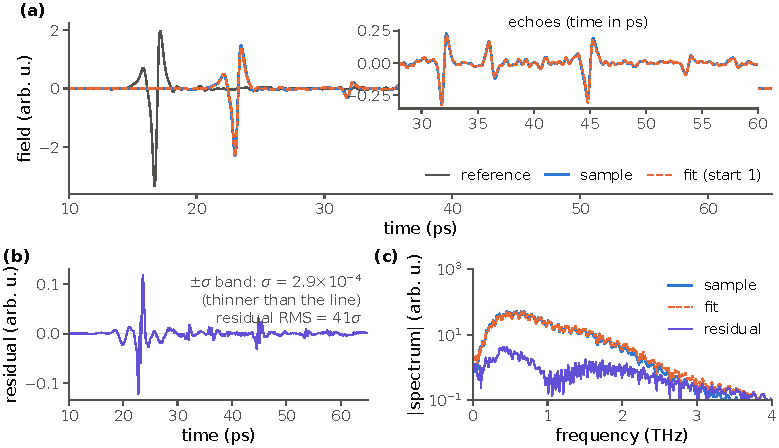
\includegraphics[width=\linewidth]{fig3_exp_fit}
  \caption{Quartz/Si (TeraSmart, 1000 waveforms in \SI{15}{\minute}, 2425 samples at \SI{33}{\femto\second}; $\sigma=\num{2.9e-4}$, peak/$\sigma=7.9\times10^3$). (a) Reference, sample, Adam fit (start 1); inset, echoes. (b) Residual ($\pm\sigma$ band thinner than the line; MAE $15\sigma$, RMS $41\sigma$). (c) Spectra.}
  \label{fig:expfit}
\end{figure}

\begin{table}[!htb]\centering\scriptsize\setlength{\tabcolsep}{2.6pt}
  \caption{Quartz/Si end points ($d$ in \si{\micro\metre}). Starts: $\nq=1.982/1.900/2.010$, $\dq=1000/900/900$, $\kq=0.0071$; Si $3.40/0.0054/400$. Adam: lowest-loss iterate (start 3); softplus, L-BFGS: start 1. Six knots: the model of Section~\ref{sec:disp} on these data, no hinge; ranges over the Si knots. Adhesive: $n\in[1.4,1.8]$ (at 1.40). rMSE change relative to row 4: $-5.0$, $-4.3$, $-57$, \SI{-59}{\percent} (rows 5--8). CR bounds grow 41-fold with the residual RMS.}
  \label{tab:exp}
  \begin{tabular}{l l cccccc}\toprule
    estimator & model & $\nq$ & $\kq$ & $\dq$ & $\nS$ & $\kS$ & $\dS$ \\\midrule
    Adam, Eq.~(\ref{eq:lossexp}) & two layers & 1.9639 & 0.00541 & 994.22 & 3.4476 & $-0.00146$ & 381.42\\
    \quad softplus & two layers & 1.9595 & 0.00478 & 996.60 & 3.4681 & $0.00011$ & 379.11\\
    L-BFGS, Eq.~(\ref{eq:lossexp}) & two layers & 1.9536 & 0.00305 & 999.59 & 3.4954 & $0.00436$ & 376.10\\
    L-BFGS, rMSE & two layers & 1.9968 & 0.00778 & 977.71 & 3.3037 & $-0.00727$ & 398.14\\
    L-BFGS, rMSE & + gap \SI{8.0}{\micro\metre} & 2.0148 & 0.00546 & 958.59 & 3.2382 & $-0.00180$ & 409.10\\
    L-BFGS, rMSE & + adhesive \SI{9.7}{\micro\metre} & 2.0132 & 0.00570 & 958.20 & 3.2439 & $-0.00229$ & 407.80\\
    L-BFGS, rMSE & six knots & & & 989.30 & 3.392--3.402 & $-0.0060$ to $-0.0030$ & 387.26\\
    L-BFGS, rMSE & knots + gap \SI{6.4}{\micro\metre} & & & 971.83 & 3.316--3.322 & $-0.0126$ to $0.0047$ & 398.31\\\midrule
    \multicolumn{2}{l}{CR bound (Adam row)} & $6.1\times10^{-5}$ & $8.7\times10^{-6}$ & 0.032 & $2.8\times10^{-4}$ & $1.9\times10^{-5}$ & 0.031\\
    \bottomrule
  \end{tabular}
\end{table}

% =====================================================================================
\section{The loss landscape of the experimental fit}\label{sec:landscape}
\subsection{What the pulse timings fix, and the two-phase descent}\label{sec:sens}
The shape of the loss near its minimum is set by the sensitivity $J_{ki}=\partial\hat y(t_k)/\partial \xi_i$ \cite{Kay1993,Aster2018} in nominal-scaled coordinates $\xi_i=(p_i-p_i^{\mathrm{opt}})/p_i^{(0)}$, whose singular values $s_1\ge\dots\ge s_6$ ($J/\sqrt L$; Fig.~\ref{fig:twophase} caption) span four decades. A counting argument explains them, for interfaces without intermediate layers. The main-pulse delay fixes $\sum_j(n_j-1)d_j$ and each echo spacing one $n_jd_j$, so together they fix $\dq+\dS$. The remaining soft $n$--$d$ direction ($s_4$) transfers thickness between the layers at constant $n_jd_j$, constrained only by the echo amplitudes: the thickness-transfer valley. The softest, $s_6$, splits a fixed attenuation $\kq\dq+\kS\dS$ between the layers: the $\kap$ valley. Within the two-layer model all sixteen end points of this paper agree on $\dq+\dS$ and both $n_jd_j$ to \SI{0.06}{\percent}, while $\dq$ spans \SI{2}{\percent} and $\kS$ changes sign; an interface layer (Table~\ref{tab:exp}) moves $\nq\dq$ by \SI{1}{\percent}.

As $T$ depends on $\kap_j$ only through $\tilde n_j$, $\lVert\partial y/\partial\kap_j\rVert=\lVert\partial y/\partial n_j\rVert$: the $\kap_j$ are two to three orders of magnitude less precise only relative to their small values.

Following Li et al.\ \cite{Li2018}, the two directions of largest spread of the visited parameter vectors (principal-component analysis, PCA) define a plane on which the loss is mapped (Fig.~\ref{fig:twophase}). In Phase~I, until every start has completed \SI{95}{\percent} of its loss decrease, each descends the well-conditioned $n$--$d$ directions; in Phase~II, \SI{92}{\percent} of the budget, all drift along the $\kap$ valley, since Adam's normalised step moves $\kap$ at the rate $\eta$ although the loss hardly changes.

\begin{figure}[!htb]\centering
  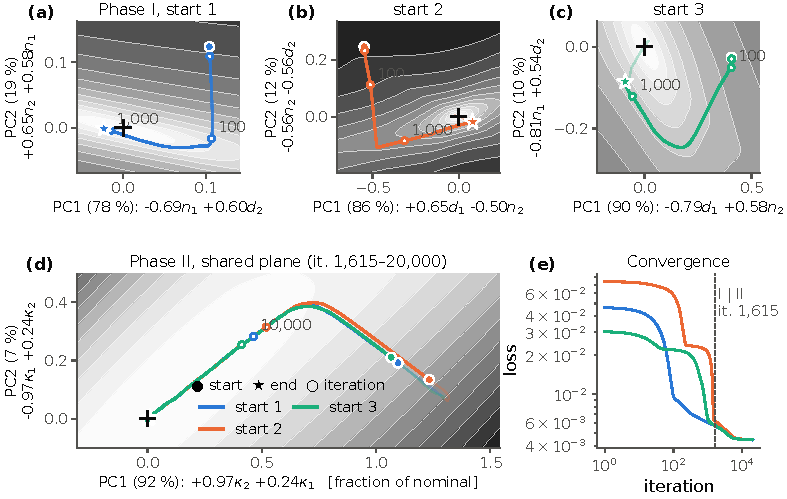
\includegraphics[width=0.95\linewidth]{fig4_adam_two_phase}
  \caption{Adam in the PCA planes of its path. Grey: log loss, lighter is lower. Axes: variance fraction and composition of each component, nominal-scaled (1 = q, 2 = Si). $+$ Adam end point, $\bullet$ start, $\star$ end of phase; path numbers: iteration. (a)--(c) Phase~I (iterations 1--1615), one plane per start, axes scaled by $\sqrt{G_{ii}}$, $G=J^\top J/L$; loss falls by 81--\SI{92}{\percent}. (d) Phase~II, shared plane, fractional coordinates (\SI{99.7}{\percent} of the variance), spanned by $\kq$, $\kS$; loss falls by 22--\SI{29}{\percent}. (e) Loss. Singular values $s_1\ldots s_6$ of $J/\sqrt L$: 8.66 (total optical thickness), 1.54 (optical thickness moved between layers), 0.69 (physical thickness at fixed delay, mainly $\dq$), 0.073 (thickness transfer), 0.019 (total attenuation), 0.0016 (attenuation split).}
  \label{fig:twophase}
\end{figure}

\subsection{Cram\'er--Rao bounds, and why the sign of $\kS$ is a model artefact}\label{sec:cr}
(i) For an exact model and white noise $\sigma$, any unbiased estimator obeys the CR bound $\mathrm{cov}(\hat \xi)\ge\sigma^2 (J^\top J)^{-1}$ \cite{Kay1993}, here at the Adam row of Table~\ref{tab:exp}. (ii) $\kS$ lies 77 bounds below zero and $\nS$ about a hundred above the literature value. But the residual RMS ($41\sigma$) far exceeds any defensible noise level, so noise can neither explain the sign nor make it significant. With bounds recomputed from the residuals (scaled by the residual RMS, or the sandwich covariance $H^{-1}J^\top\Sigma_rJH^{-1}$, $H$ the Hessian, $\Sigma_r$ the residual covariance \cite{White1980}), $|\kS|$ is below two bounds at the Adam row and 3.6--9.6 at the least-squares (L-BFGS, rMSE) row. (iii) The data fix the total attenuation; its split, the weakest direction, depends on the estimator ($\kS$ from $-0.007$ to $+0.004$). (iv) Richer models do not remove the negative sign: six knots leave $\kS<0$ across the band, a gap makes it swing from $-0.013$ to $+0.005$, and a free $\tau$ gives $\kS>0$ only with $\nS=3.64$ (we fit $\tau$ only where, as for PI, it brings a fixed-index substrate into agreement and the acquisition motivates it). Like the \SI{0.9}{\percent} excess of $\nS$, the sign is a model artefact.

Softplus imposes the sign: $\kap_j=\kap_j^{(0)}\,\mathrm{softplus}(\beta\theta_j)/\mathrm{softplus}(\beta)$, $\beta=5$, $\mathrm{softplus}(z)=\ln(1+e^z)$, which, unlike a rectifier, never freezes. It drives $\kS$ to zero at a cost of \SI{0.3}{\percent} in loss, moving $n$, $d$ along the thickness-transfer valley and $\nS$ to $+\SI{1.5}{\percent}$: the sign is fixed, not the model.

% =====================================================================================
\section{L-BFGS versus Adam}\label{sec:lbfgs}
L-BFGS runs from the same starts and loss (Fig.~\ref{fig:lbfgs}); an Adam iteration and an L-BFGS evaluation each cost one forward and backward pass. It completes Phase~I in 8--39 iterations (22--96 evaluations) and its final level in 120--150 evaluations (300 with confirming restarts). Adam reaches it in 5000--5900 iterations at $\eta=10^{-4}$ and 360--460 at $3\times10^{-3}$ (none diverging), and $4.5\times10^{-3}$, below L-BFGS's best, in 620--660: L-BFGS's advantage is needing no step size.

L-BFGS stops \SI{3.7}{\percent} above Adam's end point at a kink, not a barrier: $|\hat y_k-y_k|$ has a corner where a residual crosses zero, and along $-\nabla\Lt$ two residuals change sign, so the loss rises (one-sided slope $+0.023$ in scaled units, predicted $-0.036$), yet falls monotonically towards Adam's end point. BFGS copes with kinks under a weak-Wolfe line search, not the strong-Wolfe one here \cite{Lewis2013}. With the smooth rMSE it converges, elsewhere on the thickness-transfer valley. A frequency-domain loss term adds no information (same CR bounds, white noise, full band).

\begin{figure}[!htb]\centering
  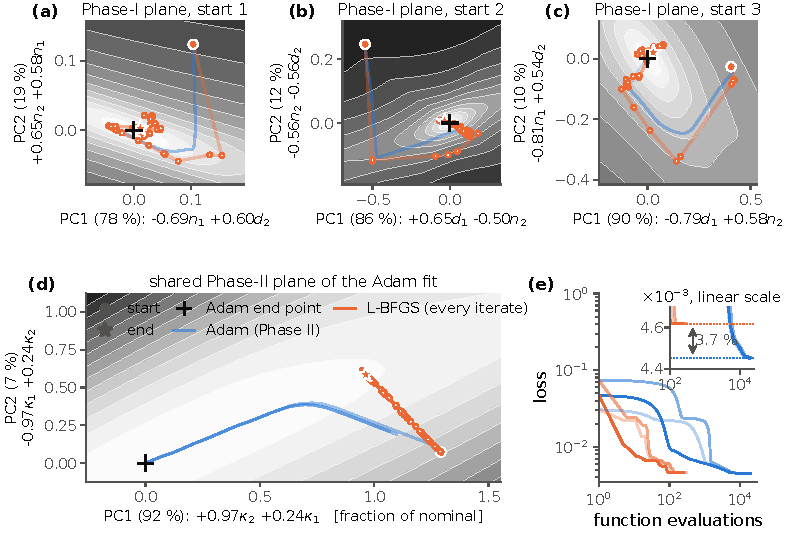
\includegraphics[width=0.95\linewidth]{fig5_lbfgs_trajectory}
  \caption{L-BFGS (orange; memory 20, $\le3$ restarts) in the planes of Fig.~\ref{fig:twophase}; Adam faint blue. (a)--(c) Phase-I planes, holding \SIrange{12}{55}{\percent} of each displacement. (d) Phase-II plane, holding \SIrange{97}{99.8}{\percent}; end points \num{0.05} off it (in $n$, $d$), \num{1.13} along it; contours are Adam's. (e) Loss, one shade per start; inset, linear. rMSE runs: gradient down six decades, starts agree to \SI{0.2}{\nano\metre}.}
  \label{fig:lbfgs}
\end{figure}

% =====================================================================================
\section{A dispersive model: quartz--air--Si with six frequency knots}\label{sec:disp}
To see what a dispersive model adds, we fit the same plates re-mounted with an air gap ($n=1$, $\kap=0$). Here $n_j(f)$, $\kap_j(f)$ are natural cubic splines through six equally spaced knots over \SIrange{0.2}{3.0}{THz} (above the noise floor), constant outside; each knot is its start value plus a trainable variable $\vartheta$ times a fixed scale $\Delta$, and a hinge $\overline{\max(0,-\kap_j(f))}$ (band mean) penalises $\kap<0$. Adam runs with each parameter's knots tied (stage~1, non-dispersive), then free (stage~2) (Figs.~\ref{fig:qasfit}, \ref{fig:qasnk}). Its $\sigma$ (3000 waveforms, \SI{115}{\pico\second}) is three times that of Section~\ref{sec:exp} as two noise bursts fall before the pulse, its white level lower (\num{2.7e-5} vs \num{4.5e-5}): multiples of $\sigma$ do not compare.

\begin{table}[!htb]\centering\scriptsize\setlength{\tabcolsep}{3.2pt}
  \caption{Quartz--air--Si knots and CR bounds; $n_jd_j$ at \SI{1}{THz} 1926.0 (q; group value 1928.2, which the echo timing measures), \SI{1319.3}{\micro\metre} (Si); $\dq$, $\dS$ correlation $-0.98$.}
  \label{tab:qas}
  \begin{tabular}{l l cccccc c c}\toprule
    $f$ (THz) & & 0.20 & 0.76 & 1.32 & 1.88 & 2.44 & 3.00 & stage 1 & CR bound\\\midrule
    quartz & $n$    & 1.9652 & 1.9712 & 1.9727 & 1.9745 & 1.9780 & 1.9917 & 1.9753 & $(4.2\text{--}7.5)\times10^{-4}$\\
           & $\kap$ & 0.0006 & 0.0034 & 0.0068 & 0.0089 & 0.0110 & 0.0114 & 0.0050 & $(0.3\text{--}6.0)\times10^{-4}$\\
    Si     & $n$    & 3.3963 & 3.3926 & 3.3928 & 3.3940 & 3.3916 & 3.3818 & 3.3903 & $(1.9\text{--}2.2)\times10^{-3}$\\
           & $\kap$ & 0.0012 & $<10^{-4}$ & 0.0009 & 0.0002 & 0.0007 & 0.0048 & 0.0002 & $(0.4\text{--}12)\times10^{-4}$\\\midrule
    \multicolumn{2}{l}{$\dq$, $d_{\mathrm{air}}$, $\dS$ (\si{\micro\metre})} & \multicolumn{6}{c}{976.6, 125.9, 388.9} & 974.5, 126.8, 389.1 & 0.221, 0.027, 0.220\\
    \bottomrule
  \end{tabular}
\end{table}

\begin{figure}[!htb]\centering
  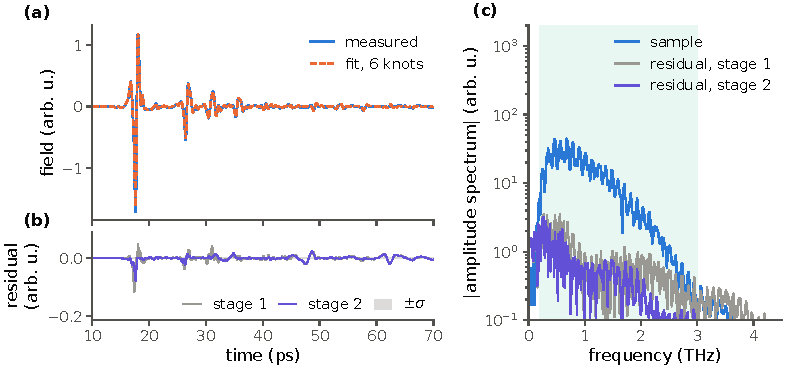
\includegraphics[width=\linewidth]{fig6_qas_fit}
  \caption{Quartz--air--Si, six knots ($\sigma=\num{9.0e-4}$, raised by pre-pulse noise bursts; white level below that of Fig.~\ref{fig:expfit}). (a) Pulse and fit; (b) residuals, stage~1 (tied) and 2 (free); (c) spectra, fit band shaded. Freeing the knots: loss $3.62\to2.93\times10^{-3}$ ($-\SI{19}{\percent}$), MAE $4.0\sigma\to3.2\sigma$.}
  \label{fig:qasfit}
\end{figure}

\begin{figure}[!htb]\centering
  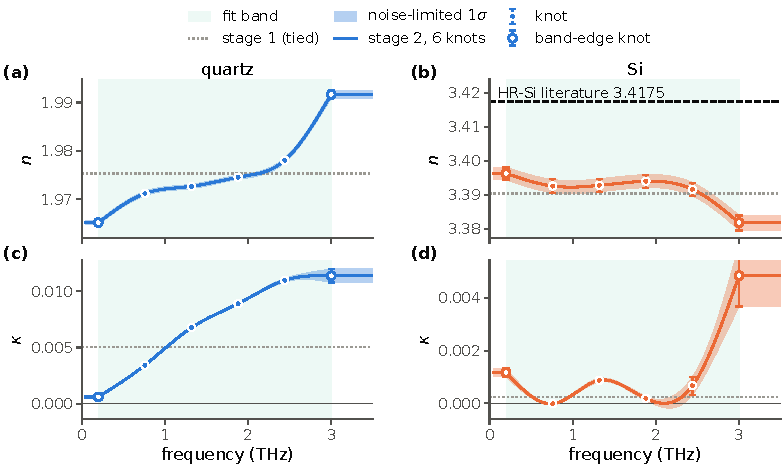
\includegraphics[width=0.9\linewidth]{fig7_qas_nk}
  \caption{Six-knot quartz--air--Si fit: (a), (b) $n(f)$, (c), (d) $\kap(f)$; stage~1 dotted. Bands: noise-limited (CR) $1\sigma$, 6.4 times wider with the residual RMS; the Si $n$ band is mostly a common offset (thickness-transfer valley), and at residual-scaled bounds the high-resistivity Si (HR-Si) value \cite{Dai2004} (dashed) is two bounds from the knot mean. Hollow: unconstrained band-edge knots.}
  \label{fig:qasnk}
\end{figure}


First, the gap, of known index, is eight times better determined than the plates (Table~\ref{tab:qas}). Second, Si is non-dispersive: tying its knots costs \SI{0.7}{\percent} in loss; their ripple (knot-grid resolution; possibly the gap etalon, $c/2d_{\mathrm{air}}\approx\SI{1.19}{THz}$) is not significant at residual-scaled bounds. A separate run without the hinge gives $\kS>0$ in stage~1, so here the positive sign comes from the modelled air gap, not dispersion. Third, the mean Si knot is \SI{0.8}{\percent} low, but the loss minimised at fixed $\nS$ varies by $<\SI{0.05}{\percent}$ over $\nS=3.38$--3.43, including the literature value.

% =====================================================================================
\section{Discussion and conclusions}\label{sec:conclusions}
A differentiable TMM measures what the pulse timings measure: each layer's $n_jd_j$ and, given time zero, the total thickness. A simulated thin film stays at the CR bound; its error in $d$ passes \SI{1}{\percent} where the round trip falls below two thirds of the pulse width. In experiments the model sets the error budget. Quartz group $\nq\dq$ differs by \SI{1.2}{\percent} between two mountings, but by \SI{0.2}{\percent} once an interface gap is modelled (time zero then accounts for $\sim$\SI{7}{\femto\second}, \SI{2.2}{\micro\metre} in $\dq+\dS$): the interface model sets the accuracy of $n_jd_j$, \SI{1}{\percent}, against a \SI{0.06}{\percent} reproducibility. Adam drifts along the attenuation split for most of its budget; L-BFGS needs no step size but stalls at a kink of the MAE. Realistic uncertainties are estimator spreads (\SI{2}{\percent} in $\dq$, \SI{6}{\percent} in $\dS$); weak absorption needs a sign constraint. Six knots leave Si non-dispersive and fix a gap eight times better than the plates. \todo{[mechanically measured thicknesses to be included]}

\begin{backmatter}
\bmsection{Funding} \todo{[to be added]}

\bmsection{Acknowledgments} \todo{[to be added]}

\bmsection{Disclosures} The authors declare no conflicts of interest. \todo{[confirm; industrial affiliation]}

\bmsection{Data availability} Traces and the notebooks regenerating every figure and number: \todo{[repository DOI]}.
\end{backmatter}

\bibliography{refs}

\end{document}
